



\documentclass[10pt,A4]{article}	



\usepackage{ragged2e}




%----------------------------------------------------------------------------------------
%	ENCODING
%----------------------------------------------------------------------------------------

% we use utf8 since we want to build from any machine
\usepackage[utf8]{inputenc}		

%----------------------------------------------------------------------------------------
%	LOGIC
%----------------------------------------------------------------------------------------

% provides \isempty test
\usepackage{xstring, xifthen}

%----------------------------------------------------------------------------------------
%	FONT BASICS
%----------------------------------------------------------------------------------------

% some tex-live fonts - choose your own

%\usepackage[defaultsans]{droidsans}
%\usepackage[default]{comfortaa}
%\usepackage{cmbright}
\usepackage[default]{raleway}
%\usepackage{fetamont}
%\usepackage[default]{gillius}
%\usepackage[light,math]{iwona}
%\usepackage[thin]{roboto} 

% set font default
\renewcommand*\familydefault{\sfdefault} 	
\usepackage[T1]{fontenc}

% more font size definitions
\usepackage{moresize}

%----------------------------------------------------------------------------------------
%	FONT AWESOME ICONS
%---------------------------------------------------------------------------------------- 

% include the fontawesome icon set
\usepackage{fontawesome}


% use to vertically center content
% credits to: http://tex.stackexchange.com/questions/7219/how-to-vertically-center-two-images-next-to-each-other
\newcommand{\vcenteredinclude}[1]{\begingroup
\setbox0=\hbox{\includegraphics{#1}}%
\parbox{\wd0}{\box0}\endgroup}

% use to vertically center content
% credits to: http://tex.stackexchange.com/questions/7219/how-to-vertically-center-two-images-next-to-each-other
\newcommand*{\vcenteredhbox}[1]{\begingroup
\setbox0=\hbox{#1}\parbox{\wd0}{\box0}\endgroup}

% icon shortcut
\newcommand{\icon}[3] { 							
	\makebox(#2, #2){\textcolor{maincol}{\csname fa#1\endcsname}}
}	

% icon with text shortcut
\newcommand{\icontext}[4]{ 						
	\vcenteredhbox{\icon{#1}{#2}{#3}}  \hspace{2pt}  \parbox{0.9\mpwidth}{\textcolor{#4}{#3}}
}

% icon with website url
\newcommand{\iconhref}[5]{ 						
    \vcenteredhbox{\icon{#1}{#2}{#5}}  \hspace{2pt} \href{#4}{\textcolor{#5}{#3}}
}

% icon with email link
\newcommand{\iconemail}[5]{ 						
    \vcenteredhbox{\icon{#1}{#2}{#5}}  \hspace{2pt} \href{mailto:#4}{\textcolor{#5}{#3}}
}

%----------------------------------------------------------------------------------------
%	PAGE LAYOUT  DEFINITIONS
%----------------------------------------------------------------------------------------

% page outer frames (debug-only)
% \usepackage{showframe}		

% we use paracol to display breakable two columns
\usepackage{paracol}

% define page styles using geometry
\usepackage[a4paper]{geometry}

% remove all possible margins
\geometry{top=1cm, bottom=1cm, left=1cm, right=1cm}

\usepackage{fancyhdr}
\pagestyle{empty}

% space between header and content
% \setlength{\headheight}{0pt}

% indentation is zero
\setlength{\parindent}{0mm}

%----------------------------------------------------------------------------------------
%	TABLE /ARRAY DEFINITIONS
%---------------------------------------------------------------------------------------- 

% extended aligning of tabular cells
\usepackage{array}

% custom column right-align with fixed width
% use like p{size} but via x{size}
\newcolumntype{x}[1]{%
>{\raggedleft\hspace{0pt}}p{#1}}%


%----------------------------------------------------------------------------------------
%	GRAPHICS DEFINITIONS
%---------------------------------------------------------------------------------------- 

%for header image
\usepackage{graphicx}

% use this for floating figures
% \usepackage{wrapfig}
% \usepackage{float}
% \floatstyle{boxed} 
% \restylefloat{figure}

%for drawing graphics		
\usepackage{tikz}				
\usetikzlibrary{shapes, backgrounds,mindmap, trees}

%----------------------------------------------------------------------------------------
%	Color DEFINITIONS
%---------------------------------------------------------------------------------------- 
\usepackage{transparent}
\usepackage{color}

% primary color
\definecolor{maincol}{RGB}{ 45, 50, 90 }
\definecolor{mainbar}{RGB}{ 50, 50, 200 }


% accent color, secondary
% \definecolor{accentcol}{RGB}{ 250, 150, 10 }

% dark color
\definecolor{darkcol}{RGB}{ 70, 70, 70 }

% light color
\definecolor{lightcol}{RGB}{245,245,245}


% Package for links, must be the last package used
\usepackage[hidelinks]{hyperref}

% returns minipage width minus two times \fboxsep
% to keep padding included in width calculations
% can also be used for other boxes / environments
\newcommand{\mpwidth}{\linewidth-\fboxsep-\fboxsep}
	


%============================================================================%
%
%	CV COMMANDS
%
%============================================================================%

%----------------------------------------------------------------------------------------
%	 CV LIST
%----------------------------------------------------------------------------------------

% renders a standard latex list but abstracts away the environment definition (begin/end)
\newcommand{\cvlist}[1] {
	\begin{itemize}{#1}\end{itemize}
}

%----------------------------------------------------------------------------------------
%	 CV TEXT
%----------------------------------------------------------------------------------------

% base class to wrap any text based stuff here. Renders like a paragraph.
% Allows complex commands to be passed, too.
% param 1: *any
\newcommand{\cvtext}[1] {
	\begin{tabular*}{1\mpwidth}{p{0.98\mpwidth}}
		\parbox{1\mpwidth}{#1}
	\end{tabular*}
}

%----------------------------------------------------------------------------------------
%	CV SECTION
%----------------------------------------------------------------------------------------

% Renders a a CV section headline with a nice underline in main color.
% param 1: section title
\newcommand{\cvsection}[1] {
	\vspace{14pt}
	\cvtext{
		\textbf{\LARGE{\textcolor{darkcol}{\uppercase{#1}}}}\\[-4pt]
		\textcolor{maincol}{ \rule{0.1\textwidth}{2pt} } \\
	}
}

%----------------------------------------------------------------------------------------
%	META SKILL
%----------------------------------------------------------------------------------------

% Renders a progress-bar to indicate a certain skill in percent.
% param 1: name of the skill / tech / etc.
% param 2: level (for example in years)
% param 3: percent, values range from 0 to 1
\newcommand{\cvskill}[3] {
	\begin{tabular*}{1\mpwidth}{p{0.72\mpwidth}  r}
 		\textcolor{black}{\textbf{#1}} & \textcolor{maincol}{#2}\\
	\end{tabular*}%
	
	\hspace{4pt}
	\begin{tikzpicture}[scale=1,rounded corners=2pt,very thin]
		\fill [lightcol] (0,0) rectangle (1\mpwidth, 0.15);
		\fill [maincol] (0,0) rectangle (#3\mpwidth, 0.15);
  	\end{tikzpicture}%
}


%----------------------------------------------------------------------------------------
%	 CV EVENT
%----------------------------------------------------------------------------------------

% Renders a table and a paragraph (cvtext) wrapped in a parbox (to ensure minimum content
% is glued together when a pagebreak appears).
% Additional Information can be passed in text or list form (or other environments).
% the work you did
% param 1: time-frame i.e. Sep 14 - Jan 15 etc.
% param 2:	 event name (job position etc.)
% param 3: Customer, Employer, Industry
% param 4: Short description
% param 5: work done (optional)
% param 6: technologies include (optional)
% param 7: achievements (optional)
\newcommand{\cvevent}[7] {
	
	% we wrap this part in a parbox, so title and description are not separated on a pagebreak
	% if you need more control on page breaks, remove the parbox
	\parbox{\mpwidth}{
		\begin{tabular*}{1\mpwidth}{p{0.72\mpwidth}  r}
	 		\Large\textcolor{black}{\textbf{#2}} & \colorbox{maincol}{\makebox[0.25\mpwidth]{\textcolor{white}{#1}}} \\
			\large\textcolor{maincol}{\textbf{#3}} & \\
		\end{tabular*}\\[4pt]
	
		\ifthenelse{\isempty{#4}}{}{
			\large\cvtext{#4}\\
		}
	}

	\ifthenelse{\isempty{#5}}{}{
		\vspace{4pt}
		{#5}
	}
	\vspace{4pt}
}

%----------------------------------------------------------------------------------------
%	 CV META EVENT
%----------------------------------------------------------------------------------------

% Renders a CV event on the sidebar
% param 1: title
% param 2: subtitle (optional)
% param 3: customer, employer, etc,. (optional)
% param 4: info text (optional)
\newcommand{\cvmetaevent}[4] {
	\textcolor{maincol} {\cvtext{\textbf{\begin{flushleft}#1\end{flushleft}}}}

	\ifthenelse{\isempty{#2}}{}{
	\textcolor{darkcol} {\cvtext{\textbf{#2}} }
	}

	\ifthenelse{\isempty{#3}}{}{
		\cvtext{{ \textcolor{darkcol} {#3} }}\\
	}

	\cvtext{#4}\\[14pt]
}

%---------------------------------------------------------------------------------------
%	QR CODE
%----------------------------------------------------------------------------------------

% Renders a qrcode image (centered, relative to the parentwidth)
% param 1: percent width, from 0 to 1
\newcommand{\cvqrcode}[1] {
	\begin{center}
		\includegraphics[width={#1}\mpwidth]{qrcode}
	\end{center}
}

%=+=+=+=+=+=+=+=+=+=+=+=+=+=+=+=+=+=+=+=+=+=+=+=+=+=+=+=+=+=+=+=+=+=+=+=+=+=+=+=+
%,,,,,,,,,,,,,,,,,,,,,,,,,,,,,,,,,,,,,,,,,,,,,,,,,,,,,,,,,,,,,,,,,,,,,,,,,,,,,,,,
                       % EDIT AFTER THIS POINT
%''''''''''''''''''''''''''''''''''''''''''''''''''''''''''''''''''''''''''''''''
%=+=+=+=+=+=+=+=+=+=+=+=+=+=+=+=+=+=+=+=+=+=+=+=+=+=+=+=+=+=+=+=+=+=+=+=+=+=+=+=+


%============================================================================%
%
%
%
%	DOCUMENT CONTENT
%
%
%
%============================================================================%
\begin{document}
\columnratio{0.31}
\setlength{\columnsep}{2.2em}
\setlength{\columnseprule}{4pt}
\colseprulecolor{lightcol}
\begin{paracol}{2}
\begin{leftcolumn}
%---------------------------------------------------------------------------------------
%	META IMAGE
%----------------------------------------------------------------------------------------
%\includegraphics[width=\linewidth]{untitled.jpg}	%trimming relative to image size



\cvsection{CONTACTO}
	
\begin{figure}
    \centering
    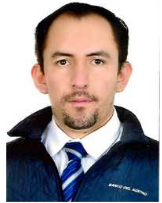
\includegraphics[width=0.25\textwidth]{./Imagenes/Foto.png}\\
    \justifying\normalsize
    Idealista, intrigado en las investigaciones científicas con fundamentos sobre el desarrollo de sistemas embebidos y seguridad tecnológica. Ingeniero en Electrónica y Comunicaciones, Magister en Ciberseguridad, con visión a la superación personal y profesional; abierto a la adquisición de nuevo conocimiento y la aplicación del mismo
\end{figure}

\icontext{Whatsapp}{14}{\href{https://wa.me/59305504123}{0995504123}}{black}\\[6pt]
\icontext{Facebook}{14}{\href{https://web.facebook.com/homjavel}{facebook.com/homjavel}}{black}\\[6pt]
\icontext{Linkedin}{14}{\href{https://www.linkedin.com/in/homero-velastegu\%C3\%AD-izurieta-8b7950160/}{Homero Velasteguí Izuierta}}{black}\\[6pt]
\iconemail{EnvelopeSquare}{14}{vehoja@gmail.com}{vehoja@gmail.com}{black}\\[6pt]
\icontext{Github}{14}{\href{https://github.com/fresvel}{fresvel}}{black}\\[6pt]
\vfill\null
%\cvqrcode{0.7}

\begin{figure}[b]
    \centering
    \href{https://wa.me/59305504123}{\includegraphics[width=0.25\textwidth]{Imagenes/w_qr.png}}
    \\ {Contactar}
    
\end{figure}




\begin{figure}
    \centering
    \href{https://mega.nz/file/dWp31RrK#z9XoP_M5yQvO3shsg4i-p4wTlL0G3Oc5KjafktydL9M}{\includegraphics[width=0.25\textwidth]{Imagenes/cv_qr.png}}
    \\ {Descargar CV}
\end{figure}

\end{leftcolumn}


\begin{rightcolumn}
%---------------------------------------------------------------------------------------
%	TITLE  HEADER
%----------------------------------------------------------------------------------------
\begin{center}
\Huge{ \textbf{{ { Homero Javier Velasteguí Izurieta} } } } \\    
\end{center}


\fcolorbox{white}{mainbar}{\begin{minipage}[c][2cm][c]{1\mpwidth}
	\begin {center}
        %[-24pt]		
		%\textcolor{white}{ \rule{0.1\textwidth}{1.25pt} } \\[4pt]
		\large{ \textcolor{white} {Ingeniero en Electrónica \& Comunicaciones - Magister en Cibersegurida } }
		
	\end {center}
\end{minipage}}\\[14pt] 

\vspace{-12pt}

%---------------------------------------------------------------------------------------
%	EDUCATION
%----------------------------------------------------------------------------------------
%\vfill\null


\cvsection{EDUCACIÓN}

\cvevent
	{\textbf{2020 - 2021}}
	{Magister en Ciberseguridad}
	{Pontificia Universidad Católica - Ambato (Ecuador)}
	{Publicación: "IoT-based Security Alarm Protocol"}
\vfill\null

\cvevent
	{\textbf{20XX - 20XX}}
	{M. Tech. - Computer Science $\&$ Engineering}
	{University Name - City, State (Country)}
	{Passed with \textbf{X.XX CGPA}. Thesis work on Your thesis domain.}
\vfill\null

\cvevent
    {\textbf{20XX - 20XX}}
    {B. Tech. - Information Technology}
    {University Name - City, State (Country)}
    {Passed with \textbf{XX.XX$\%$}. Major project was Major project name.}
\vfill\null

%---------------------------------------------------------------------------------------
%	WORK EXPERIENCE
%----------------------------------------------------------------------------------------
\vfill\null
\cvsection{WORK EXPERIENCE}

\cvevent
	{\textbf{Jan YY - Dec YY}}
	{Position name}
	{Institute/Organization, City (State)}
	{Write about your roles and responsibilities. In case of teaching experience also write about the subjects you taught.}
	{}
\vfill\null

\cvevent
	{\textbf{Jan YY - Jul YY}}
	{Position name}
	{Institute/Organization, City (State)}
	{Write about your roles and responsibilities. In case of teaching experience also write about the subjects you taught.}
	{}
\vfill\null
%---------------------------------------------------------------------------------------
%	PUBLICATION
%----------------------------------------------------------------------------------------
\vspace{-0.5cm}
\vfill\null
\cvsection{PUBLICATIONS}

\cvevent
	{\textbf{UGC Listed}}
	{Title of your research paper}
	{Journal Name (ISSN: XXXX-XXXX) Vol XX, Issue XX, 20XX}
	{Status: Accepted and Published}
	{}
\vfill\null

\cvevent
	{\textbf{SCI - IF X.XXX}}
	{Title of your research paper}
	{Journal Name (ISSN: XXXX-XXXX) Vol XX, Issue XX, 20XX}
	{Status: Under Review}
	{}
\vfill\null

\cvevent
	{\textbf{SCI - IF X.XXX}}
	{Title of your research paper}
	{Journal Name (ISSN: XXXX-XXXX) Vol XX, Issue XX, 20XX}
	{Status: Under Review}
	{}
\vfill\null

\end{rightcolumn}
\end{paracol}




%---------------------------------------------------------------------------------------
%	PROJECTS
%----------------------------------------------------------------------------------------
\vfill\null
\cvsection{PROJECTS}

\cvevent
	{\textbf{20XX}}
	{Project Name}
	{Tool: Python, Raspberry Pi}
	{A short description of your project.}
\vfill\null


\cvevent
	{\textbf{20XX}}
	{Project Name}
	{Tool: Web Development}
	{A short description of your project.}
\vfill\null


\cvevent
	{\textbf{20XX}}
	{Project Name}
	{Tool: Android Studio}
	{A short description of your project.}
\vfill\null

%---------------------------------------------------------------------------------------
%	WORKSHOPS
%----------------------------------------------------------------------------------------
\vfill\null
\cvsection{WORKSHOPS \& CONFERENCES}

\cvevent
	{\textbf{Mon 20XX}}
	{Name of Conference}
	{Conducted by}
	{}
\vfill\null

\cvevent
	{\textbf{May 2019}}
	{IEEE Internation Conference on Future of Internet of Things}
	{IEEE \& IIT Kanpur}
	{}
\vfill\null

\cvevent
	{\textbf{Jul 2020}}
	{Online International Workshop on Machine Learning Applications to Images, IoT and Wireless Sensor Networks}
	{University of Essex and IIIT, Lucknow}
	{}
\vfill\null
%---------------------------------------------------------------------------------------
%	SKILLS
%----------------------------------------------------------------------------------------

%---------------------------------------------------------------------------------------
%	PERSONAL DETAILS
%----------------------------------------------------------------------------------------
\vfill\null
\cvsection{EXTRACURRICULAR}
\vspace{-0.3cm}
\begin{itemize}
  \item Put all the points that are not covered in \textbf{above sections}.
  \item Put all the points that are \textbf{not covered} in above sections.
  \item Put all the \textbf{points} that are not covered in above sections.
  \item \textbf{Put all the points} that are not covered in above sections.
\end{itemize}
\vfill\null


% hotfixes to create fake-space to ensure the whole height is used
\vfill
\vfill
\vfill


\newpage



\end{document}















































\usepackage{ragged2e}
\usepackage{wrapfig}




%----------------------------------------------------------------------------------------
%	ENCODING
%----------------------------------------------------------------------------------------

% we use utf8 since we want to build from any machine
\usepackage[utf8]{inputenc}		

%----------------------------------------------------------------------------------------
%	LOGIC
%----------------------------------------------------------------------------------------

% provides \isempty test
\usepackage{xstring, xifthen}

%----------------------------------------------------------------------------------------
%	FONT BASICS
%----------------------------------------------------------------------------------------

% some tex-live fonts - choose your own

%\usepackage[defaultsans]{droidsans}
%\usepackage[default]{comfortaa}
%\usepackage{cmbright}
\usepackage[default]{raleway}
%\usepackage{fetamont}
%\usepackage[default]{gillius}
%\usepackage[light,math]{iwona}
%\usepackage[thin]{roboto} 

% set font default
\renewcommand*\familydefault{\sfdefault} 	
\usepackage[T1]{fontenc}

% more font size definitions
\usepackage{moresize}

%----------------------------------------------------------------------------------------
%	FONT AWESOME ICONS
%---------------------------------------------------------------------------------------- 

% include the fontawesome icon set
\usepackage{fontawesome}


% use to vertically center content
% credits to: http://tex.stackexchange.com/questions/7219/how-to-vertically-center-two-images-next-to-each-other
\newcommand{\vcenteredinclude}[1]{\begingroup
\setbox0=\hbox{\includegraphics{#1}}%
\parbox{\wd0}{\box0}\endgroup}

% use to vertically center content
% credits to: http://tex.stackexchange.com/questions/7219/how-to-vertically-center-two-images-next-to-each-other
\newcommand*{\vcenteredhbox}[1]{\begingroup
\setbox0=\hbox{#1}\parbox{\wd0}{\box0}\endgroup}

% icon shortcut
\newcommand{\icon}[3] { 							
	\makebox(#2, #2){\textcolor{maincol}{\csname fa#1\endcsname}}
}	

% icon with text shortcut
\newcommand{\icontext}[4]{ 						
	\vcenteredhbox{\icon{#1}{#2}{#3}}  \hspace{2pt}  \parbox{0.9\mpwidth}{\textcolor{#4}{#3}}
}

% icon with website url
\newcommand{\iconhref}[5]{ 						
    \vcenteredhbox{\icon{#1}{#2}{#5}}  \hspace{2pt} \href{#4}{\textcolor{#5}{#3}}
}

% icon with email link
\newcommand{\iconemail}[5]{ 						
    \vcenteredhbox{\icon{#1}{#2}{#5}}  \hspace{2pt} \href{mailto:#4}{\textcolor{#5}{#3}}
}

%----------------------------------------------------------------------------------------
%	PAGE LAYOUT  DEFINITIONS
%----------------------------------------------------------------------------------------

% page outer frames (debug-only)
% \usepackage{showframe}		

% we use paracol to display breakable two columns
\usepackage{paracol}

% define page styles using geometry
\usepackage[a4paper]{geometry}

% remove all possible margins
\geometry{top=1cm, bottom=1cm, left=1cm, right=1cm}

\usepackage{fancyhdr}
\pagestyle{empty}

% space between header and content
% \setlength{\headheight}{0pt}

% indentation is zero
\setlength{\parindent}{0mm}

%----------------------------------------------------------------------------------------
%	TABLE /ARRAY DEFINITIONS
%---------------------------------------------------------------------------------------- 

% extended aligning of tabular cells
\usepackage{array}

% custom column right-align with fixed width
% use like p{size} but via x{size}
\newcolumntype{x}[1]{%
>{\raggedleft\hspace{0pt}}p{#1}}%


%----------------------------------------------------------------------------------------
%	GRAPHICS DEFINITIONS
%---------------------------------------------------------------------------------------- 

%for header image
\usepackage{graphicx}

% use this for floating figures
% \usepackage{wrapfig}
% \usepackage{float}
% \floatstyle{boxed} 
% \restylefloat{figure}

%for drawing graphics		
\usepackage{tikz}				
\usetikzlibrary{shapes, backgrounds,mindmap, trees}

%----------------------------------------------------------------------------------------
%	Color DEFINITIONS
%---------------------------------------------------------------------------------------- 
\usepackage{transparent}
\usepackage{color}

% primary color
\definecolor{maincol}{RGB}{ 45, 50, 90 }
\definecolor{mainbar}{RGB}{ 50, 50, 200 }


% accent color, secondary
% \definecolor{accentcol}{RGB}{ 250, 150, 10 }

% dark color
\definecolor{darkcol}{RGB}{ 70, 70, 70 }

% light color
\definecolor{lightcol}{RGB}{245,245,245}


% Package for links, must be the last package used
\usepackage[hidelinks]{hyperref}

% returns minipage width minus two times \fboxsep
% to keep padding included in width calculations
% can also be used for other boxes / environments
\newcommand{\mpwidth}{\linewidth-\fboxsep-\fboxsep}
	


%============================================================================%
%
%	CV COMMANDS
%
%============================================================================%

%----------------------------------------------------------------------------------------
%	 CV LIST
%----------------------------------------------------------------------------------------

% renders a standard latex list but abstracts away the environment definition (begin/end)
\newcommand{\cvlist}[1] {
	\begin{itemize}{#1}\end{itemize}
}

%----------------------------------------------------------------------------------------
%	 CV TEXT
%----------------------------------------------------------------------------------------

% base class to wrap any text based stuff here. Renders like a paragraph.
% Allows complex commands to be passed, too.
% param 1: *any
\newcommand{\cvtext}[1] {
	\begin{tabular*}{1\mpwidth}{p{0.98\mpwidth}}
		\parbox{1\mpwidth}{#1}
	\end{tabular*}
}

%----------------------------------------------------------------------------------------
%	CV SECTION
%----------------------------------------------------------------------------------------

% Renders a a CV section headline with a nice underline in main color.
% param 1: section title
\newcommand{\cvsection}[1] {
	\vspace{14pt}
	\cvtext{
		\textbf{\LARGE{\textcolor{darkcol}{\uppercase{#1}}}}\\[-4pt]
		\textcolor{maincol}{ \rule{0.1\textwidth}{2pt} } \\
	}
}

%----------------------------------------------------------------------------------------
%	META SKILL
%----------------------------------------------------------------------------------------

% Renders a progress-bar to indicate a certain skill in percent.
% param 1: name of the skill / tech / etc.
% param 2: level (for example in years)
% param 3: percent, values range from 0 to 1
\newcommand{\cvskill}[3] {
	\begin{tabular*}{1\mpwidth}{p{0.72\mpwidth}  r}
 		\textcolor{black}{\textbf{#1}} & \textcolor{maincol}{#2}\\
	\end{tabular*}%
	
	\hspace{4pt}
	\begin{tikzpicture}[scale=1,rounded corners=2pt,very thin]
		\fill [lightcol] (0,0) rectangle (1\mpwidth, 0.15);
		\fill [maincol] (0,0) rectangle (#3\mpwidth, 0.15);
  	\end{tikzpicture}%
}


%----------------------------------------------------------------------------------------
%	 CV EVENT
%----------------------------------------------------------------------------------------

% Renders a table and a paragraph (cvtext) wrapped in a parbox (to ensure minimum content
% is glued together when a pagebreak appears).
% Additional Information can be passed in text or list form (or other environments).
% the work you did
% param 1: time-frame i.e. Sep 14 - Jan 15 etc.
% param 2:	 event name (job position etc.)
% param 3: Customer, Employer, Industry
% param 4: Short description
% param 5: work done (optional)
% param 6: technologies include (optional)
% param 7: achievements (optional)
\newcommand{\cvevent}[7] {
	
	% we wrap this part in a parbox, so title and description are not separated on a pagebreak
	% if you need more control on page breaks, remove the parbox
	\parbox{\mpwidth}{
		\begin{tabular*}{1\mpwidth}{p{0.72\mpwidth}  r}
	 		\Large\textcolor{black}{\textbf{#2}} & \colorbox{maincol}{\makebox[0.25\mpwidth]{\textcolor{white}{#1}}} \\
			\large\textcolor{maincol}{\textbf{#3}} & \\
		\end{tabular*}\\[4pt]
	
		\ifthenelse{\isempty{#4}}{}{
			\large\cvtext{#4}\\
		}
	}

	\ifthenelse{\isempty{#5}}{}{
		\vspace{4pt}
		{#5}
	}
	\vspace{4pt}
}

%----------------------------------------------------------------------------------------
%	 CV META EVENT
%----------------------------------------------------------------------------------------

% Renders a CV event on the sidebar
% param 1: title
% param 2: subtitle (optional)
% param 3: customer, employer, etc,. (optional)
% param 4: info text (optional)
\newcommand{\cvmetaevent}[4] {
	\textcolor{maincol} {\cvtext{\textbf{\begin{flushleft}#1\end{flushleft}}}}

	\ifthenelse{\isempty{#2}}{}{
	\textcolor{darkcol} {\cvtext{\textbf{#2}} }
	}

	\ifthenelse{\isempty{#3}}{}{
		\cvtext{{ \textcolor{darkcol} {#3} }}\\
	}

	\cvtext{#4}\\[14pt]
}

%---------------------------------------------------------------------------------------
%	QR CODE
%----------------------------------------------------------------------------------------

% Renders a qrcode image (centered, relative to the parentwidth)
% param 1: percent width, from 0 to 1
\newcommand{\cvqrcode}[1] {
	\begin{center}
		\includegraphics[width={#1}\mpwidth]{qrcode}
	\end{center}
}

%=+=+=+=+=+=+=+=+=+=+=+=+=+=+=+=+=+=+=+=+=+=+=+=+=+=+=+=+=+=+=+=+=+=+=+=+=+=+=+=+
%,,,,,,,,,,,,,,,,,,,,,,,,,,,,,,,,,,,,,,,,,,,,,,,,,,,,,,,,,,,,,,,,,,,,,,,,,,,,,,,,
                       % EDIT AFTER THIS POINT
%''''''''''''''''''''''''''''''''''''''''''''''''''''''''''''''''''''''''''''''''
%=+=+=+=+=+=+=+=+=+=+=+=+=+=+=+=+=+=+=+=+=+=+=+=+=+=+=+=+=+=+=+=+=+=+=+=+=+=+=+=+


%============================================================================%
%
%
%
%	DOCUMENT CONTENT
%
%
%
%============================================================================%
\begin{document}
\columnratio{0.31}
\setlength{\columnsep}{2.2em}
\setlength{\columnseprule}{4pt}
\colseprulecolor{lightcol}

\begin{paracol}{2}

\begin{leftcolumn}

    

    \icontext{Whatsapp}{14}{\href{https://wa.me/59305504123}{0995504123}}{black}\\[6pt]
    \icontext{Facebook}{14}{\href{https://web.facebook.com/homjavel}{facebook.com/homjavel}}{black}\\[6pt]
    \icontext{Linkedin}{14}{\href{https://www.linkedin.com/in/homero-velastegu\%C3\%AD-izurieta-8b7950160/}{Homero Velasteguí Izuierta}}{black}\\[6pt]
    \iconemail{EnvelopeSquare}{14}{vehoja@gmail.com}{vehoja@gmail.com}{black}\\[6pt]
    \icontext{Github}{14}{\href{https://github.com/fresvel}{fresvel}}{black}\\[6pt]
    \vfill\null
    %\cvqrcode{0.7}

\end{leftcolumn}

\begin{rightcolumn}
    
    



    \begin{figure}[t]
        
        \href{https://wa.me/59305504123}{\includegraphics[width=0.1\textwidth]{Imagenes/w_qr.png}}
        \\ {Contactar}
        
    \end{figure}




\end{rightcolumn}

\end{paracol}











\fcolorbox{white}{mainbar}{
\begin{minipage}[c][2cm][c]{1\mpwidth}
	\begin {center}
        %[-24pt]		
		%\textcolor{white}{ \rule{0.1\textwidth}{1.25pt} } \\[4pt]
		\huge{ \textbf{\textcolor{white} {Homero Javier Velasteguí Izurieta } }}
		
	\end {center}
\end{minipage}}\\[14pt] 


\begin{paracol}{2}
\begin{leftcolumn}
%---------------------------------------------------------------------------------------
%	META IMAGE
%----------------------------------------------------------------------------------------
%\includegraphics[width=\linewidth]{untitled.jpg}	%trimming relative to image size



    \begin{figure}[t]
        
        \href{https://wa.me/59305504123}{\includegraphics[width=0.1\textwidth]{Imagenes/w_qr.png}}
        \\ {Contactar}
        
    \end{figure}

\begin{center}
\Huge{ \textbf{{ { Homero Javier Velasteguí Izurieta} } } } \\    
\end{center}


	
\begin{figure}
    \centering
    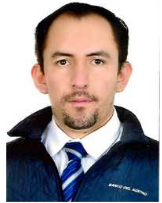
\includegraphics[width=0.25\textwidth]{./Imagenes/Foto.png}\\
    \justifying\normalsize
    Idealista, intrigado en las investigaciones científicas con fundamentos sobre el desarrollo de sistemas embebidos y seguridad tecnológica. Ingeniero en Electrónica y Comunicaciones, Magister en Ciberseguridad, con visión a la superación personal y profesional; abierto a la adquisición de nuevo conocimiento y la aplicación del mismo
\end{figure}








\begin{figure}
    \centering
    \href{https://mega.nz/file/dWp31RrK#z9XoP_M5yQvO3shsg4i-p4wTlL0G3Oc5KjafktydL9M}{\includegraphics[width=0.25\textwidth]{Imagenes/cv_qr.png}}
    \\ {Descargar CV}
\end{figure}

\end{leftcolumn}


\begin{rightcolumn}
%---------------------------------------------------------------------------------------
%	TITLE  HEADER
%----------------------------------------------------------------------------------------



\fcolorbox{white}{mainbar}{\begin{minipage}[c][2cm][c]{1\mpwidth}
	\begin {center}
        %[-24pt]		
		%\textcolor{white}{ \rule{0.1\textwidth}{1.25pt} } \\[4pt]
		\large{ \textcolor{white} {Ingeniero en Electrónica \& Comunicaciones - Magister en Cibersegurida } }
		
	\end {center}
\end{minipage}}\\[14pt] 

\vspace{-12pt}

%---------------------------------------------------------------------------------------
%	EDUCATION
%----------------------------------------------------------------------------------------
%\vfill\null


\cvsection{EDUCACIÓN}

\cvevent
	{\textbf{2020 - 2021}}
	{Magister en Ciberseguridad}
	{Pontificia Universidad Católica - Ambato (Ecuador)}
	{Publicación: "IoT-based Security Alarm Protocol"}
\vfill\null

\cvevent
	{\textbf{20XX - 20XX}}
	{M. Tech. - Computer Science $\&$ Engineering}
	{University Name - City, State (Country)}
	{Passed with \textbf{X.XX CGPA}. Thesis work on Your thesis domain.}
\vfill\null

\cvevent
    {\textbf{20XX - 20XX}}
    {B. Tech. - Information Technology}
    {University Name - City, State (Country)}
    {Passed with \textbf{XX.XX$\%$}. Major project was Major project name.}
\vfill\null

%---------------------------------------------------------------------------------------
%	WORK EXPERIENCE
%----------------------------------------------------------------------------------------
\vfill\null
\cvsection{WORK EXPERIENCE}

\cvevent
	{\textbf{Jan YY - Dec YY}}
	{Position name}
	{Institute/Organization, City (State)}
	{Write about your roles and responsibilities. In case of teaching experience also write about the subjects you taught.}
	{}
\vfill\null

\cvevent
	{\textbf{Jan YY - Jul YY}}
	{Position name}
	{Institute/Organization, City (State)}
	{Write about your roles and responsibilities. In case of teaching experience also write about the subjects you taught.}
	{}
\vfill\null
%---------------------------------------------------------------------------------------
%	PUBLICATION
%----------------------------------------------------------------------------------------
\vspace{-0.5cm}
\vfill\null
\cvsection{PUBLICATIONS}

\cvevent
	{\textbf{UGC Listed}}
	{Title of your research paper}
	{Journal Name (ISSN: XXXX-XXXX) Vol XX, Issue XX, 20XX}
	{Status: Accepted and Published}
	{}
\vfill\null

\cvevent
	{\textbf{SCI - IF X.XXX}}
	{Title of your research paper}
	{Journal Name (ISSN: XXXX-XXXX) Vol XX, Issue XX, 20XX}
	{Status: Under Review}
	{}
\vfill\null

\cvevent
	{\textbf{SCI - IF X.XXX}}
	{Title of your research paper}
	{Journal Name (ISSN: XXXX-XXXX) Vol XX, Issue XX, 20XX}
	{Status: Under Review}
	{}
\vfill\null

\end{rightcolumn}
\end{paracol}




%---------------------------------------------------------------------------------------
%	PROJECTS
%----------------------------------------------------------------------------------------
\vfill\null
\cvsection{PROJECTS}

\cvevent
	{\textbf{20XX}}
	{Project Name}
	{Tool: Python, Raspberry Pi}
	{A short description of your project.}
\vfill\null


\cvevent
	{\textbf{20XX}}
	{Project Name}
	{Tool: Web Development}
	{A short description of your project.}
\vfill\null


\cvevent
	{\textbf{20XX}}
	{Project Name}
	{Tool: Android Studio}
	{A short description of your project.}
\vfill\null

%---------------------------------------------------------------------------------------
%	WORKSHOPS
%----------------------------------------------------------------------------------------
\vfill\null
\cvsection{WORKSHOPS \& CONFERENCES}

\cvevent
	{\textbf{Mon 20XX}}
	{Name of Conference}
	{Conducted by}
	{}
\vfill\null

\cvevent
	{\textbf{May 2019}}
	{IEEE Internation Conference on Future of Internet of Things}
	{IEEE \& IIT Kanpur}
	{}
\vfill\null

\cvevent
	{\textbf{Jul 2020}}
	{Online International Workshop on Machine Learning Applications to Images, IoT and Wireless Sensor Networks}
	{University of Essex and IIIT, Lucknow}
	{}
\vfill\null
%---------------------------------------------------------------------------------------
%	SKILLS
%----------------------------------------------------------------------------------------

%---------------------------------------------------------------------------------------
%	PERSONAL DETAILS
%----------------------------------------------------------------------------------------
\vfill\null
\cvsection{EXTRACURRICULAR}
\vspace{-0.3cm}
\begin{itemize}
  \item Put all the points that are not covered in \textbf{above sections}.
  \item Put all the points that are \textbf{not covered} in above sections.
  \item Put all the \textbf{points} that are not covered in above sections.
  \item \textbf{Put all the points} that are not covered in above sections.
\end{itemize}
\vfill\null


% hotfixes to create fake-space to ensure the whole height is used
\vfill
\vfill
\vfill


\newpage

On the other side, if you are only interested on
certain values you can use the contour plot, you 
can use the contour plot, you can use the contour 
plot, you can use the contour plot, you can use 
the contour plot, you can use the contour plot, 
you can use the contour plot, like the one on the left.On the other side, if you are only interested on
certain values you can use the contour plot, you 
can use the contour plot, you can use the contour 
plot, you can use the contour plot, you can use 
the contour plot, you can use the contour plot, 
you can use the contour plot, like the one on the left.On the other side, if you are only interested on
certain values you can use the contour plot, you 
can use the contour plot, you can use the contour 
plot, you can use the contour plot, you can use 
the contour plot, you can use the contour plot, 
you can use the contour plot, like the one on the left.On the other side, if you are only interested on
certain values you can use the contour plot, you 
can use the contour plot, you can use the contour 
plot, you can use the contour plot, you can use 
the contour plot, you can use the contour plot, 
you can use the contour plot, like the one on the left.On the other side, if you are only interested on
certain values you can use the contour plot, you 
can use the contour plot, you can use the contour 
plot, you can use the contour plot, you can use 
the contour plot, you can use the contour plot, 
you can use the contour plot, like the one on the left.


\begin{wrapfigure}{l}{0.25\textwidth}
    \centering
    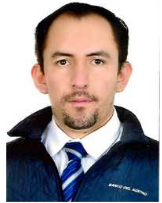
\includegraphics[width=0.25\textwidth]{./Imagenes/Foto.png}
\end{wrapfigure}


\end{document}

























%---------------------------------------------------------------------------------------
%	META SKILLS
%----------------------------------------------------------------------------------------
\cvsection{SKILLS}

%\cvskill{Skill_Name} {Years of experience} {percentage of bar fill} \\[-2pt]

\cvskill{Internet of Things} {5+ yrs} {1} \\[-2pt]

\cvskill{Machine Learning} {1+ yrs} {0.2} \\[-2pt]

\cvskill{Python} {3+ yrs} {0.6} \\[-2pt]

\cvskill{C++} {5+ yrs} {1} \\[-2pt]

\cvskill{Linux} {1+ yrs} {0.2} \\[-2pt]

\cvskill{Web Development} {5+ yrs} {1} \\[-2pt]

\cvskill{Quantum Computing} {1+ yrs} {0.2} \\[-2pt]

\cvskill{Teaching} {3+ yrs} {0.6} \\[-2pt]

%\vfill\null
%\cvqrcode{0.7}



%---------------------------------------------------------------------------------------
%	ACHIEVEMENTS
%----------------------------------------------------------------------------------------

\cvsection{ACHIEVEMENTS}

\cvmetaevent
{GATE}
{Computer Science and Information Technology (CS)}
{}
{Qualified in 2016 with 389 score in general category.}

\cvmetaevent
{IELTS}
{7.0 out of 9 Band}
{}
{A certificate issued by International Development Program (IDP), Australia to prove English language proficiency for non-native English language speakers.}

\cvmetaevent
{Cloud Computing 101}
{94.30\%}
{}
{A certificate issued by coursera to prove basic understanding of cloud computing.}

\cvmetaevent
{Achievement}
{Certificate Detail}
{}
{Description will go here as a sentence.}